% 图 84.7 —— 由 `checks/emit_hand.py` 自动拼出（probe 精测 + prims2 图元分解）
%%
% ⚠ 这是**稿子不是成品**：跑 `checks/checkhand.py 84.7` 看指标 + 看叠合图。
%%
%% ⚠ 待核：
%   · 本图 probe 报出阴影族 1 个 —— **本脚本不生成阴影**（要照原书手写）；prims2 的 strokes 里可能含阴影线，核对时留意别画重
%   · 可疑字形 1 项（空心圈 ⊙ 常被认成字母 o）—— 见文件末
%%
\documentclass[12pt]{standalone}
\usepackage{fontspec}
\setsansfont{Arial}
\newfontfamily\mfallback{DejaVu Sans}
\usepackage{tikz}
\begin{document}
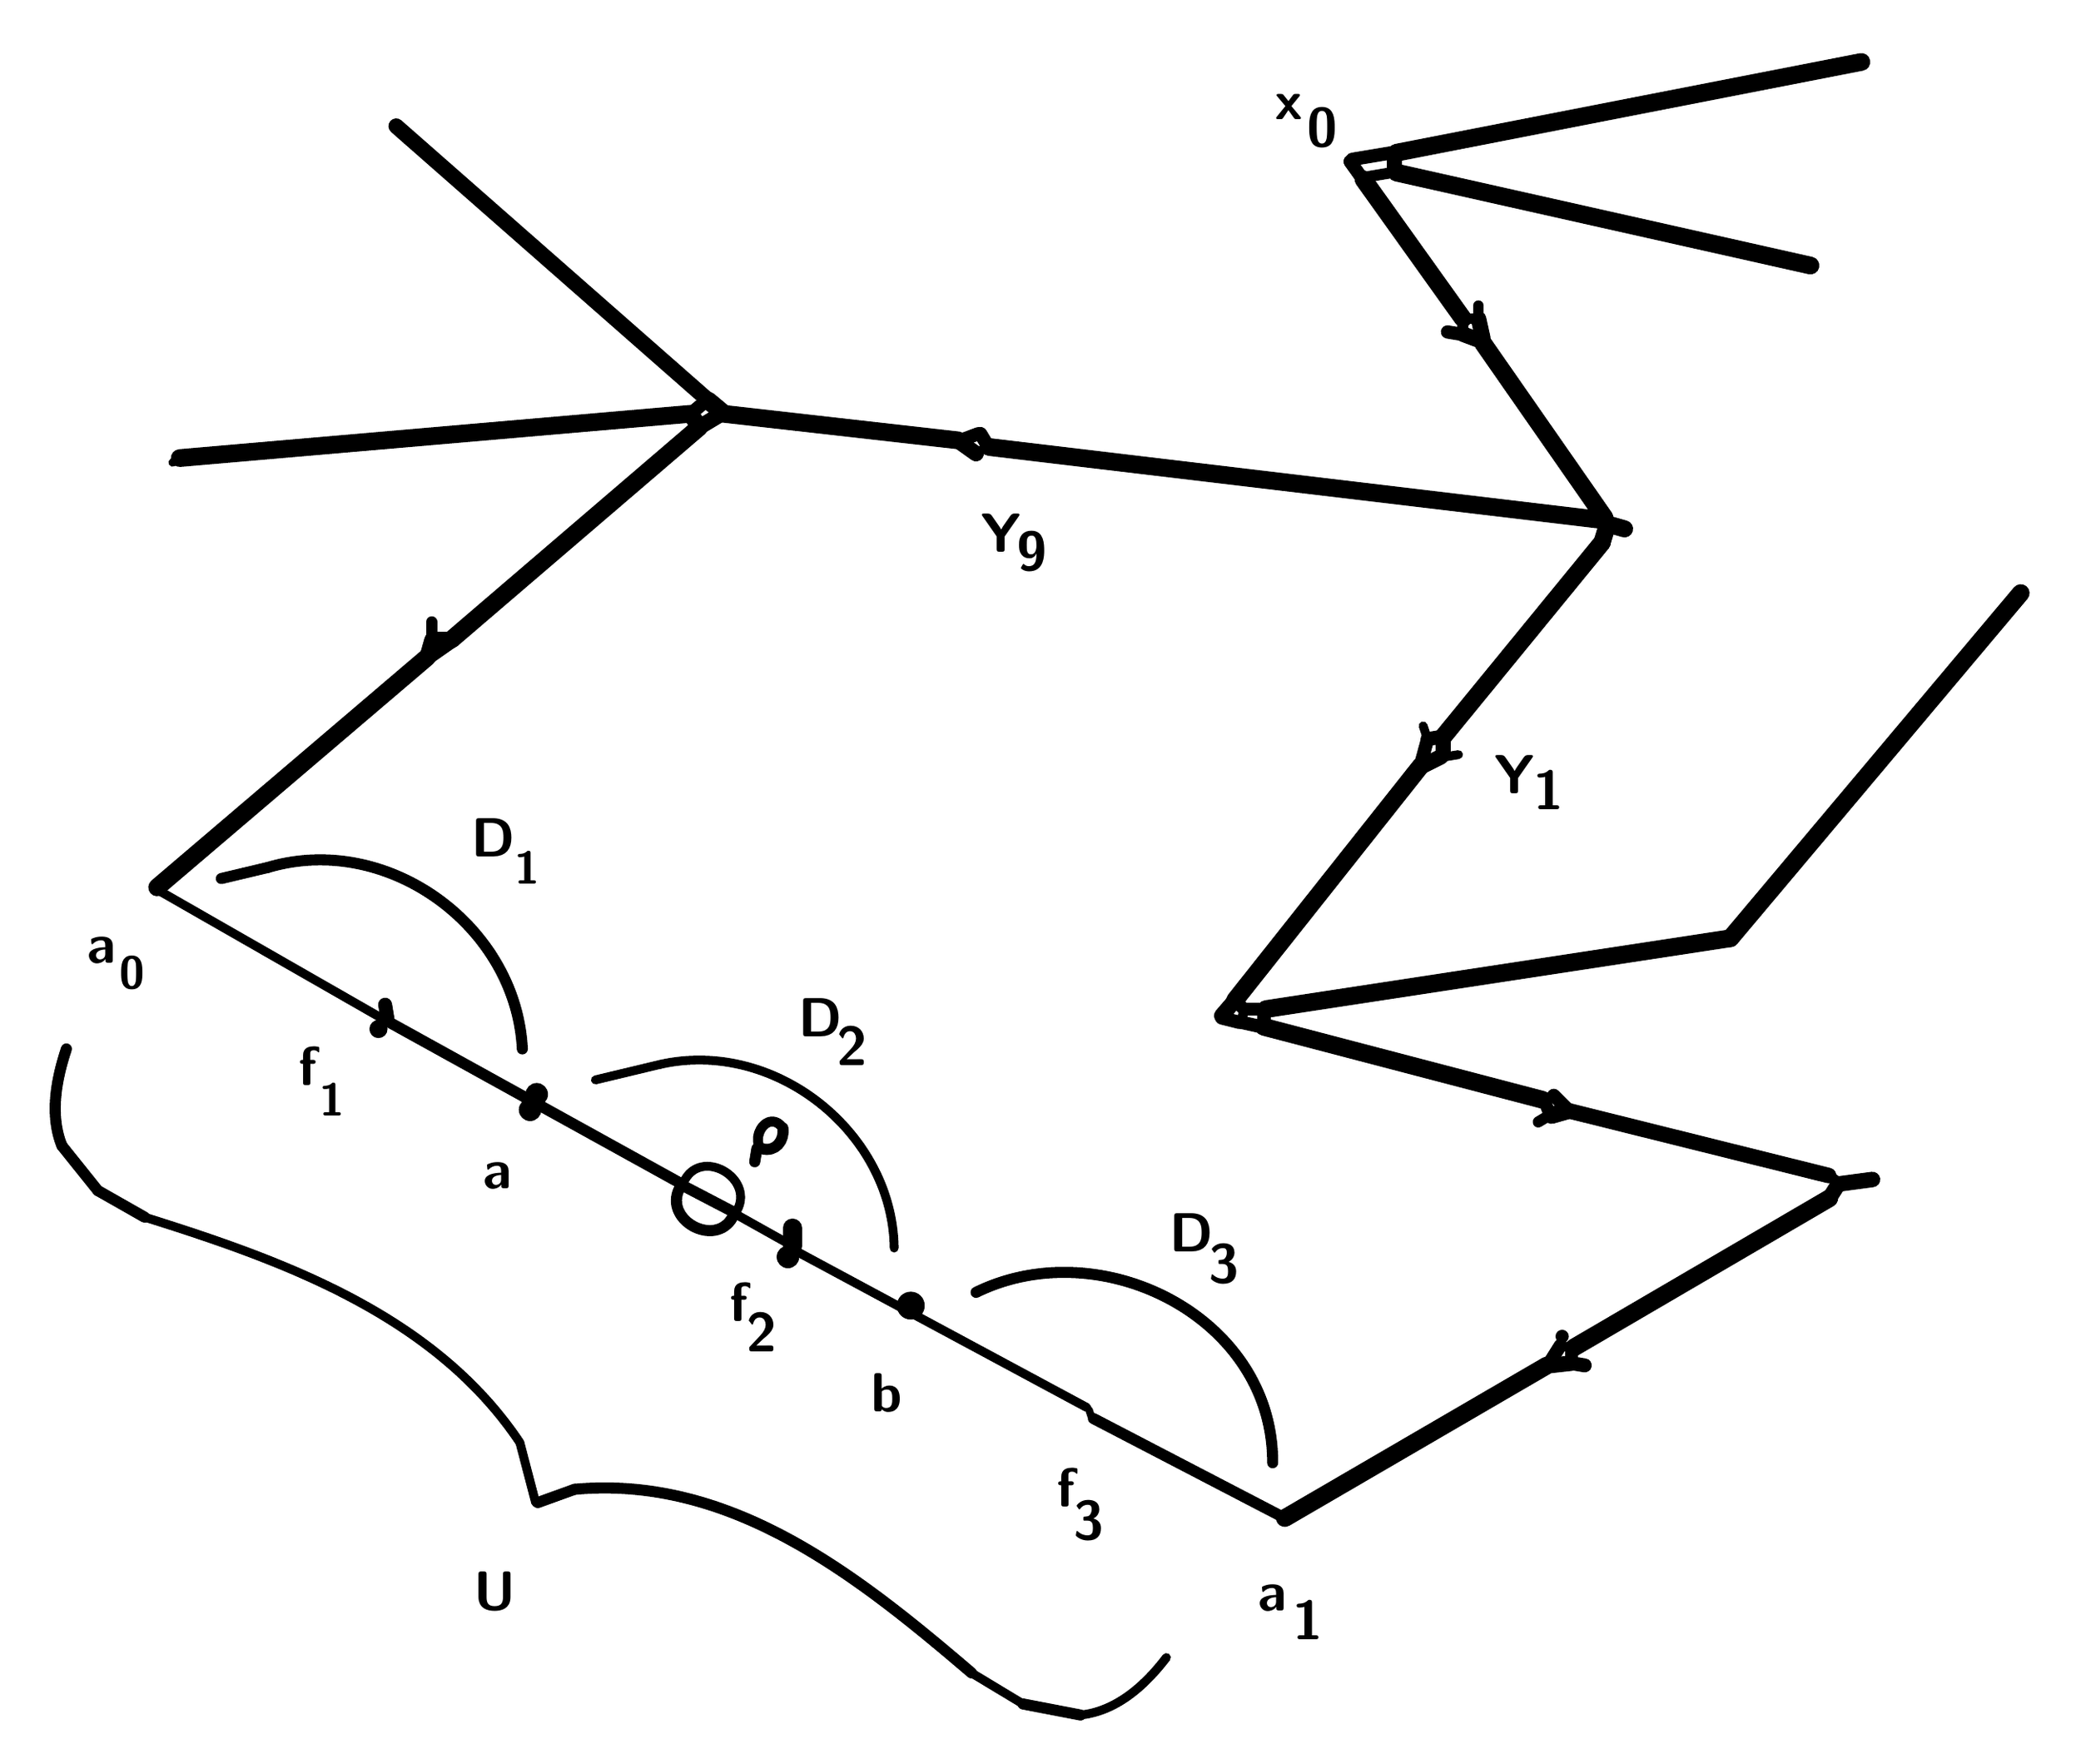
\begin{tikzpicture}[x=1pt, y=-1pt, line width=8.7pt, line cap=round, line join=round]

  %% ════ 填充区（prims2 的 fills）════

  %% ════ 直线段（prims2 的 strokes）════
  \draw[line width=8.7pt] (348.0,545.0) -- (348.0,553.0);
  \draw[line width=3.8pt] (688.0,487.0) -- (691.0,485.0);
  \draw[line width=8.0pt] (689.0,607.0) -- (570.5,676.0);
  \draw[line width=5.0pt] (570.5,676.0) -- (484.0,631.0);
  \draw[line width=7.0pt] (836.0,523.0) -- (821.0,525.0);
  \draw[line width=3.8pt] (68.0,199.0) -- (71.2,197.0);
  \draw[line width=8.0pt] (71.2,197.0) -- (302.0,177.0);
  \draw[line width=6.0pt] (700.0,606.0) -- (700.0,600.0);
  \draw[line width=7.0pt] (700.0,606.0) -- (691.0,607.0);
  \draw[line width=6.3pt] (700.0,606.0) -- (706.0,607.0);
  \draw[line width=7.0pt] (186.0,279.0) -- (193.0,279.0);
  \draw[line width=6.1pt] (436.0,191.0) -- (433.0,186.0);
  \draw[line width=6.0pt] (695.0,598.0) -- (690.0,606.0);
  \draw[line width=4.3pt] (695.0,598.0) -- (699.0,599.0);
  \draw[line width=6.3pt] (164.0,444.0) -- (165.0,450.0);
  \draw[line width=7.0pt] (542.0,449.0) -- (548.0,442.0);
  \draw[line width=7.0pt] (620.0,60.0) -- (620.0,67.0);
  \draw[line width=3.4pt] (483.0,630.0) -- (482.0,627.0);
  \draw[line width=6.0pt] (632.0,335.0) -- (635.0,324.0);
  \draw[line width=5.0pt] (652.0,134.0) -- (657.0,134.0);
  \draw[line width=6.0pt] (302.0,177.0) -- (308.0,172.0);
  \draw[line width=7.5pt] (302.0,177.0) -- (306.0,183.0);
  \draw[line width=8.0pt] (183.0,287.0) -- (61.0,391.0);
  \draw[line width=8.0pt] (548.0,442.0) -- (632.0,336.0);
  \draw[line width=5.7pt] (548.0,442.0) -- (552.0,446.0);
  \draw[line width=7.8pt] (716.0,228.0) -- (713.8,235.2);
  \draw[line width=8.0pt] (713.8,235.2) -- (642.0,323.0);
  \draw[line width=5.0pt] (685.0,497.0) -- (690.0,494.0);
  \draw[line width=7.7pt] (724.0,229.0) -- (717.0,227.0);
  \draw[line width=7.7pt] (698.0,492.0) -- (691.0,494.0);
  \draw[line width=8.0pt] (310.0,171.0) -- (316.0,176.0);
  \draw[line width=6.0pt] (650.0,141.0) -- (644.0,140.0);
  \draw[line width=7.0pt] (633.0,336.0) -- (641.0,332.0);
  \draw[line width=5.7pt] (690.0,493.0) -- (688.0,488.0);
  \draw[line width=4.0pt] (232.0,669.0) -- (224.9,641.9);
  \draw[line width=5.0pt] (55.3,540.0) -- (34.2,528.0);
  \draw[line width=5.0pt] (34.2,528.0) -- (18.0,507.8);
  \draw[line width=8.0pt] (561.0,454.0) -- (687.0,487.0);
  \draw[line width=4.0pt] (481.0,626.0) -- (349.0,555.0);
  \draw[line width=5.0pt] (332.0,509.0) -- (331.0,515.0);
  \draw[line width=5.0pt] (651.0,140.0) -- (651.0,135.0);
  \draw[line width=5.0pt] (322.0,538.0) -- (299.0,526.0);
  \draw[line width=8.0pt] (808.0,110.0) -- (621.0,68.0);
  \draw[line width=7.0pt] (431.0,195.0) -- (424.0,190.0);
  \draw[line width=6.0pt] (424.0,189.0) -- (432.0,186.0);
  \draw[line width=4.0pt] (288.2,471.0) -- (259.0,478.0);
  \draw[line width=4.2pt] (435.0,192.0) -- (432.0,195.0);
  \draw[line width=7.0pt] (169.0,47.0) -- (309.0,170.0);
  \draw[line width=5.0pt] (619.0,68.0) -- (607.0,70.0);
  \draw[line width=4.0pt] (323.0,539.0) -- (348.0,553.0);
  \draw[line width=6.0pt] (619.0,59.0) -- (601.0,62.0);
  \draw[line width=4.3pt] (551.0,451.0) -- (552.0,447.0);
  \draw[line width=7.0pt] (306.0,183.0) -- (316.0,177.0);
  \draw[line width=8.0pt] (306.0,183.0) -- (194.0,279.0);
  \draw[line width=7.0pt] (659.0,144.0) -- (651.0,141.0);
  \draw[line width=8.0pt] (437.0,192.0) -- (714.0,225.0);
  \draw[line width=7.0pt] (658.0,134.0) -- (660.0,143.0);
  \draw[line width=6.5pt] (185.0,279.0) -- (183.0,286.0);
  \draw[line width=8.0pt] (621.0,59.0) -- (831.0,18.0);
  \draw[line width=5.0pt] (478.2,765.0) -- (452.2,760.0);
  \draw[line width=4.0pt] (452.2,760.0) -- (429.0,746.0);
  \draw[line width=5.0pt] (249.6,663.0) -- (233.0,669.0);
  \draw[line width=8.0pt] (903.0,258.0) -- (771.8,414.0);
  \draw[line width=8.0pt] (771.8,414.0) -- (562.0,446.0);
  \draw[line width=6.0pt] (600.0,63.0) -- (605.0,70.0);
  \draw[line width=8.0pt] (651.0,134.0) -- (606.0,71.0);
  \draw[line width=6.0pt] (692.0,485.0) -- (698.0,491.0);
  \draw[line width=6.0pt] (551.0,452.0) -- (560.0,454.0);
  \draw[line width=6.3pt] (641.0,323.0) -- (635.0,324.0);
  \draw[line width=4.5pt] (658.0,128.0) -- (658.0,133.0);
  \draw[line width=5.0pt] (111.0,382.0) -- (90.0,387.0);
  \draw[line width=6.0pt] (184.0,287.0) -- (194.0,280.0);
  \draw[line width=4.0pt] (164.0,451.0) -- (61.0,392.0);
  \draw[line width=7.0pt] (642.0,324.0) -- (642.0,331.0);
  \draw[line width=7.0pt] (699.0,492.0) -- (816.2,521.2);
  \draw[line width=4.9pt] (816.2,521.2) -- (820.0,524.0);
  \draw[line width=4.0pt] (635.0,324.0) -- (633.0,318.0);
  \draw[line width=8.0pt] (317.0,177.0) -- (423.0,189.0);
  \draw[line width=8.0pt] (660.0,145.0) -- (715.0,224.0);
  \draw[line width=4.0pt] (649.0,331.0) -- (643.0,332.0);
  \draw[line width=5.0pt] (298.0,525.0) -- (166.0,452.0);
  \draw[line width=6.0pt] (542.0,450.0) -- (550.0,452.0);
  \draw[line width=5.0pt] (185.0,271.0) -- (185.0,278.0);
  \draw[line width=6.0pt] (561.0,453.0) -- (561.0,447.0);
  \draw[line width=6.9pt] (820.0,526.0) -- (816.5,531.5);
  \draw[line width=8.0pt] (816.5,531.5) -- (701.0,599.0);
  \draw[line width=6.0pt] (560.0,446.0) -- (553.0,446.0);

  %% ════ 曲线（prims2 的 curves —— 三段式，坐标同为 (y,x)）════
  \draw[line width=4.0pt] (224.9,641.9) .. controls (186.1,583.8) and (117.1,559.4) .. (55.3,540.0);
  \draw[line width=5.0pt] (18.0,507.8) .. controls (12.3,493.8) and (15.5,477.5) .. (20.0,464.0);
  \draw[line width=4.0pt] (323.0,537.0) .. controls (331.1,522.2) and (306.5,508.2) .. (299.0,524.0);
  \draw[line width=4.0pt] (394.0,554.0) .. controls (393.3,501.9) and (340.3,459.2) .. (288.2,471.0);
  \draw[line width=5.0pt] (334.0,509.0) .. controls (340.4,511.0) and (344.6,505.3) .. (343.7,499.7);
  \draw[line width=4.5pt] (343.7,499.7) .. controls (338.1,492.1) and (330.3,501.0) .. (333.0,508.0);
  \draw[line width=4.0pt] (517.0,739.0) .. controls (507.1,752.0) and (494.2,763.3) .. (478.2,765.0);
  \draw[line width=5.0pt] (429.0,746.0) .. controls (377.4,701.9) and (320.3,656.5) .. (249.6,663.0);
  \draw[line width=5.0pt] (431.0,574.0) .. controls (487.4,546.3) and (565.2,585.2) .. (565.0,651.0);
  \draw[line width=5.0pt] (226.0,464.0) .. controls (223.2,408.5) and (165.1,365.9) .. (111.0,382.0);
  \draw[line width=5.0pt] (321.0,540.0) .. controls (313.3,554.0) and (289.7,541.5) .. (297.0,527.0);

  %% ════ 实心点 ════
  \fill (161.0,455.0) circle (4.1);
  \fill (232.5,484.5) circle (5.1);
  \fill (229.5,491.5) circle (5.1);
  \fill (346.0,558.0) circle (5.1);
  \fill (401.5,580.0) circle (6.3);
  \fill (695.8,593.9) circle (3.0);

  %% ════ 标签（probe 直接给的 \node 行）════
  %% ⚠ 全部补了 fill=white：文字在最上层，否则与曲线交叉干扰
     \node[anchor=center,inner sep=0pt,fill=white,font=\fontsize{30.1}{37.6}\selectfont] at (572.5,38.5) {\textsf{\textbf{\textit{x}}}};   % box(563,28,17,17)
     \node[anchor=center,inner sep=0pt,fill=white,font=\fontsize{23.8}{29.8}\selectfont] at (587.5,47.7) {\textsf{\textbf{0}}};   % box(580,39,11,17)
     \node[anchor=center,inner sep=0pt,fill=white,font=\fontsize{28.7}{35.9}\selectfont] at (442.5,231.0) {\textsf{\textbf{\textit{Y}}}};   % box(434,218,16,24)
     \node[anchor=center,inner sep=0pt,fill=white,font=\fontsize{24.4}{30.5}\selectfont] at (456.4,239.1) {\textsf{\textbf{9}}};   % box(449,230,12,17)
     \node[anchor=center,inner sep=0pt,fill=white,font=\fontsize{28.7}{35.9}\selectfont] at (674.5,340.0) {\textsf{\textbf{\textit{Y}}}};   % box(666,327,16,24)
     \node[anchor=center,inner sep=0pt,fill=white,font=\fontsize{23.7}{29.7}\selectfont] at (689.8,347.4) {\textsf{\textbf{1}}};   % box(683,339,8,16)
     \node[anchor=center,inner sep=0pt,fill=white,font=\fontsize{30.3}{37.9}\selectfont] at (212.8,368.5) {\textsf{\textbf{\textit{D}}}};   % box(201,357,20,22)
     \node[anchor=center,inner sep=0pt,fill=white,font=\fontsize{22.2}{27.8}\selectfont] at (228.1,382.4) {\textsf{\textbf{1}}};   % box(222,374,7,16)
     \node[anchor=center,inner sep=0pt,fill=white,font=\fontsize{32.9}{41.1}\selectfont] at (36.1,419.6) {\textsf{\textbf{\textit{a}}}};   % box(27,409,16,18)
     \node[anchor=center,inner sep=0pt,fill=white,font=\fontsize{22.7}{28.4}\selectfont] at (49.9,429.7) {\textsf{\textbf{0}}};   % box(43,421,10,17)
     \node[anchor=center,inner sep=0pt,fill=white,font=\fontsize{31.0}{38.8}\selectfont] at (360.8,450.0) {\textsf{\textbf{\textit{D}}}};   % box(349,438,20,23)
     \node[anchor=center,inner sep=0pt,fill=white,font=\fontsize{23.6}{29.6}\selectfont] at (375.1,462.9) {\textsf{\textbf{2}}};   % box(369,454,11,17)
     \node[anchor=center,inner sep=0pt,fill=white,font=\fontsize{29.1}{36.4}\selectfont] at (130.0,472.0) {\textsf{\textbf{\textit{f}}}};   % box(124,460,11,23)
     \node[anchor=center,inner sep=0pt,fill=white,font=\fontsize{21.5}{26.9}\selectfont] at (140.0,486.9) {\textsf{\textbf{1}}};   % box(134,479,7,15)
     \node[anchor=center,inner sep=0pt,fill=white,font=\fontsize{32.9}{41.1}\selectfont] at (215.1,521.6) {\textsf{\textbf{\textit{a}}}};   % box(206,511,16,18)
     \node[anchor=center,inner sep=0pt,fill=white,font=\fontsize{31.8}{39.7}\selectfont] at (528.4,547.0) {\textsf{\textbf{\textit{D}}}};   % box(516,535,21,23)
     \node[anchor=center,inner sep=0pt,fill=white,font=\fontsize{23.0}{28.7}\selectfont] at (542.9,561.1) {\textsf{\textbf{3}}};   % box(537,552,11,17)
     \node[anchor=center,inner sep=0pt,fill=white,font=\fontsize{28.5}{35.6}\selectfont] at (325.0,578.5) {\textsf{\textbf{\textit{f}}}};   % box(319,567,11,22)
     \node[anchor=center,inner sep=0pt,fill=white,font=\fontsize{22.9}{28.7}\selectfont] at (334.1,592.4) {\textsf{\textbf{2}}};   % box(328,584,11,16)
     \node[anchor=center,inner sep=0pt,fill=white,font=\fontsize{30.0}{37.5}\selectfont] at (390.8,619.2) {\textsf{\textbf{\textit{b}}}};   % box(381,607,17,22)
     \node[anchor=center,inner sep=0pt,fill=white,font=\fontsize{29.7}{37.2}\selectfont] at (472.5,662.5) {\textsf{\textbf{\textit{f}}}};   % box(466,651,12,22)
     \node[anchor=center,inner sep=0pt,fill=white,font=\fontsize{23.0}{28.7}\selectfont] at (481.9,677.1) {\textsf{\textbf{3}}};   % box(476,668,11,17)
     \node[anchor=center,inner sep=0pt,fill=white,font=\fontsize{33.9}{42.3}\selectfont] at (213.5,708.9) {\textsf{\textbf{\textit{U}}}};   % box(202,695,23,25)
     \node[anchor=center,inner sep=0pt,fill=white,font=\fontsize{32.0}{40.0}\selectfont] at (565.1,712.1) {\textsf{\textbf{\textit{a}}}};   % box(556,702,16,17)
     \node[anchor=center,inner sep=0pt,fill=white,font=\fontsize{23.7}{29.7}\selectfont] at (580.8,722.4) {\textsf{\textbf{1}}};   % box(574,714,8,16)

  % 钉死画布：否则超出的图元/控制点会把页面撑大，1:1 回比就失准
  \pgfresetboundingbox
  \path[use as bounding box] (0,0) rectangle (920,777);
\end{tikzpicture}
\end{document}

% ⚠ 待核清单（probe 拿不准，人眼过一遍）：
%   · 未识别/跳过：⑤ 跳过/未识别的字形
